\documentclass[12pt]{report}
\usepackage[utf8]{inputenc}
\usepackage[russian]{babel}
%\usepackage[14pt]{extsizes}
\usepackage{listings}
\usepackage{graphicx}
\lstset{extendedchars=\true}
\usepackage{amsmath,amsfonts,amssymb,amsthm,mathtools} 
\usepackage{pgfplots}
\usepackage{filecontents}
\usepackage{float}
\usepackage{comment}
\usepackage{indentfirst}
\usepackage{eucal}
\usepackage{enumitem}
%s\documentclass[openany]{book}
\frenchspacing

\usepackage{indentfirst} % Красная строка

\usetikzlibrary{datavisualization}
\usetikzlibrary{datavisualization.formats.functions}

\usepackage{amsmath}


% Для листинга кода:
\lstset{ %
	language=c,                 % выбор языка для подсветки (здесь это С)
	basicstyle=\small\sffamily, % размер и начертание шрифта для подсветки кода
	numbers=left,               % где поставить нумерацию строк (слева\справа)
	numberstyle=\tiny,           % размер шрифта для номеров строк
	stepnumber=1,                   % размер шага между двумя номерами строк
	numbersep=5pt,                % как далеко отстоят номера строк от подсвечиваемого кода
	showspaces=false,            % показывать или нет пробелы специальными отступами
	showstringspaces=false,      % показывать или нет пробелы в строках
	showtabs=false,             % показывать или нет табуляцию в строках
	frame=single,              % рисовать рамку вокруг кода
	tabsize=2,                 % размер табуляции по умолчанию равен 2 пробелам
	captionpos=t,              % позиция заголовка вверху [t] или внизу [b] 
	breaklines=true,           % автоматически переносить строки (да\нет)
	breakatwhitespace=false, % переносить строки только если есть пробел
	escapeinside={\#*}{*)}   % если нужно добавить комментарии в коде
}


\usepackage[left=2cm,right=2cm, top=2cm,bottom=2cm,bindingoffset=0cm]{geometry}
% Для измененных титулов глав:
\usepackage{titlesec, blindtext, color} % подключаем нужные пакеты
\definecolor{gray75}{gray}{0.75} % определяем цвет
\newcommand{\hsp}{\hspace{20pt}} % длина линии в 20pt
% titleformat определяет стиль
\titleformat{\chapter}[hang]{\Huge\bfseries}{\thechapter\hsp\textcolor{gray75}{|}\hsp}{0pt}{\Huge\bfseries}


% plot
\usepackage{pgfplots}
\usepackage{filecontents}
\usetikzlibrary{datavisualization}
\usetikzlibrary{datavisualization.formats.functions}

\begin{document}
	%\def\chaptername{} % убирает "Глава"

\chapter*{Мои заметки про zram и память в ядре}

\section*{Литература} 

\begin{itemize}
	\item Linux. Системное программирование (Роберт Лав), глава 12, 14, 15, 16 -- с этого начинать, книга в целом лёгкая на подъем (но нужны какие-то базовые знания по ядру). Указаные главы конкретно про память, лучше читать с начала.
	\item Драйверы Устройств Linux, 3-я редакция -- сложно, но надо
	\item Ядро Linux (Бовет Д., Чезати М.) -- пока не читал. Говорят немного устаревшее, но раскрываются основные идеи памяти в ядре
	\item In-kernel memory compression -- https://lwn.net/Articles/545244/
	\item zram docs -- https://www.kernel.org/doc/Documentation/blockdev/zram.txt
\end{itemize}

\section*{Kernel memory}


\subsection*{Всякое разное про пейджы} 

\subsubsection{struct page}

Физическая страница памяти описывается структурой \texttt{struct page}. В ядре есть большой линейный массив, который содержит все структуры. То есть, существует некоторые массив хранящий \textbf{описание} (это важно) всех физических страниц. И к этим \textbf{описаниям} можно обратиться. Но, не каждый struct page можно замапить на виртуальную память - то есть описание существует страницы существует всегда, но вот обратиться к этой странице можно не всегда. Это зависит от состояния системы и от всяких других тонких моментов. 

\subsubsection{huge pages}

huge pages - это пейджы, которые больше 4кб. Аллоцировать их можно только на boottime, например передав загрузчику параметры для ядра. Они непрерывные. Например, если аллоцировать страницу на 1 гигабайт - будет залочен 1 гигабайт физический памяти под эту страницу. Описывается так же с помощью struct page.

Поддерживает это не каждый процессор, и при этом должна быть включён специальный параметр в ядре. \texttt{/sys/kernel/mm/hugepages/} - всякая инфа про них в системе

\subsubsection{idle pages}

У \texttt{struct page} есть поле \texttt{\_count} - счётчик ссылок на страницу. Если на страницу никто не ссылается, то счётчик равен 0 или отрицательный (неожиданно), поэтому чтобы проверить, используется ли сейчас страница, например, каким-нибудь процессом, нужно вызывать \texttt{page\_count()} - если 0, то страница такая страница называется idle (никем не используется), если != 0 то значит где-то используется.

\subsection*{Адресация, mmap и прочее}

\subsubsection{mmap}

mmap -- системный вызов с помощью которого мапится память устройства в пользовательскую память. 

У каждого устройства есть драйвер. Если разработчик устройства хочет, чтобы его память можно было замапить, он должен самостоятельно реализовать mmap для своего устройства и для этого есть всякое разное API.

\subsubsection{Типы адресов}

\begin{figure}[H]
	\begin{center}
		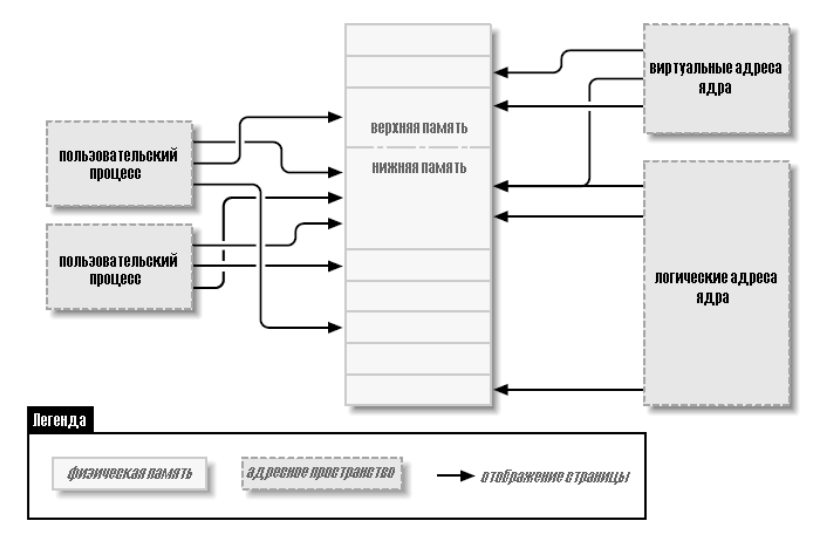
\includegraphics[scale=0.5]{img/memory.png}
	\end{center}
	\label{fig:memory}
\end{figure}

\begin{itemize}
	\item Пользовательские виртуальные адреса - это понятно;
	\item физические адреса - это тоже;
	\item адреса шин - адреса, используемые между периферийными шинами и памятью. До конца не понятно, что это такое;
	\item логические адреса ядра - это сложно;
	\item виртуальные адреса ядра - и это тоже.
\end{itemize}

Суть в том что это всё абстракции над одним и тем же куском железа (памятью).

\subsubsection{Нижняя и верхняя память}

\begin{itemize}
	\item Нижняя память -- память, для которой существуют логические адреса в пространстве ядра;
	\item верхняя память -- память для которой логические адреса не существуют, потому что она выходит за рамки диапазона адресов, отведённых для виртуальных адресов ядра.
\end{itemize}

\subsection*{DMA}

\subsubsection{Что это вообще такое?}

\begin{figure}[H]
	\begin{center}
		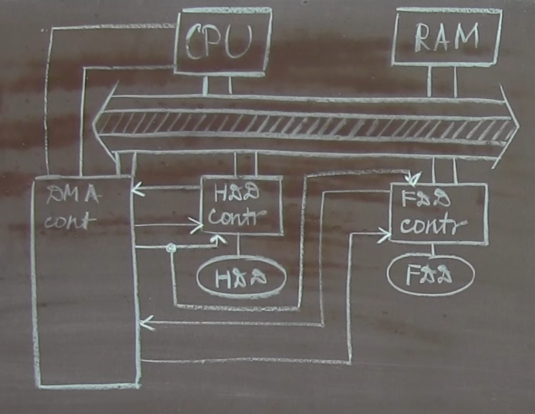
\includegraphics[scale=0.6]{img/dma-cpu.png}
	\end{center}
	\label{fig:1}
\end{figure}

Когда мы хотим прочитать что-то с устройства (речь о блочных устройствах):

\begin{itemize}
	\item CPU обращается к контроллеру устройства;
	\item читает данные;
	\item кладёт данные на шину;
	\item по шине они идут в RAM.
\end{itemize}

Direct memory access (DMA) -- грубо говоря, с помощью этой штуки можно обращаться к памяти без использования CPU. Существует DMA controller -- некоторая физическая штука, которая ставится в устройстве вместе со всем остальным. Происходит это примерно так (на примере чтения данных, для записи тоже самое):

\begin{itemize}
	\item DMA controller шлёт запрос к CPU о том что он хочет почитать устройство;
	\item CPU отсылает сигнал - что-то типа "окей, можешь читать";
	\item выставляются какие-то сигналы между контроллером DMA и контроллером устройства (это не так важно);
	\item DMA controller начинает читать данные и ставить их на шину;
	\item нужно отметить, что шина заблокирована для CPU, и он туда писать ничего не может;
	\item когда DMA controller поставил на шину весь блок данных, они уже идут в RAM;
	\item обмен сигналами между CPU и DMA controller что чтение успешно завершено (чтоб CPU уже знал, что ему можно если что вдруг лезть на шину памяти)
\end{itemize}

\subsubsection{В ядре}

todo

\section*{zRam}

zram -- модуль ядра, позволяющий жать страницы памяти прямо в оперативной памяти (в отличи от zswap, который жмёт те страницы, которые будут отправлены в swap устройство). Жмёт он только страницы размеров 4096, о чём говорит вот этот кусок кода (zram\_drv.c):

\begin{lstlisting}[language=c]
src = zs_map_object(zram->mem_pool, handle, ZS_MM_RO);
if (size == PAGE_SIZE) {
	dst = kmap_atomic(page);
	memcpy(dst, src, PAGE_SIZE);
	kunmap_atomic(dst);
	ret = 0;
} else {
	dst = kmap_atomic(page);
	ret = zcomp_decompress(zstrm, src, size, dst);
	kunmap_atomic(dst);
	zcomp_stream_put(zram->comp);
}
\end{lstlisting}

\subsection*{Как он работает}

\subsubsection*{zsmalloc}

У zram есть свой аллокатор -- zsmalloc. Хорошо работает в условиях нехватки памяти. Особенности:

\begin{itemize}
	\item аллоцирировать объекты он может только размера не больше PAGE\_SIZE - если запросить больше, то \texttt{zs\_malloc()} возвращает ошибку;
	\item \texttt{zs\_malloc()} \textbf{не возвращет} указатель, который можно разыменовать. Он возвращает некоторый дескриптор (unsinged long), который описывает аллоцированный объект;
	\item чтобы сконвертить этот дескриптор в область памяти, в которую уже можно писать/читать, нужно вызывать \texttt{zs\_map\_object()}. Это связано с тем, что на 32-битных машинах virtual address area сильно ограничен (память короче экономят на древних машинах).
\end{itemize}

\subsubsection{Структуры данных}

Драйвер описывается структурой \texttt{struct zram}:

\begin{lstlisting}[language=c]
struct zram {
	struct zram_table_entry *table;
	struct zs_pool *mem_pool;
	struct zcomp *comp;
	struct gendisk *disk;
	/* Prevent concurrent execution of device init */
	struct rw_semaphore init_lock;
	/*
	* the number of pages zram can consume for storing compressed data
	*/
	unsigned long limit_pages;
	
	struct zram_stats stats;
	/*
	* This is the limit on amount of *uncompressed* worth of data
	* we can store in a disk.
	*/
	u64 disksize;	/* bytes */
	char compressor[CRYPTO_MAX_ALG_NAME];
	/*
	* zram is claimed so open request will be failed
	*/
	bool claim; /* Protected by disk->open_mutex */
	#ifdef CONFIG_ZRAM_WRITEBACK
	struct file *backing_dev;
	spinlock_t wb_limit_lock;
	bool wb_limit_enable;
	u64 bd_wb_limit;
	struct block_device *bdev;
	unsigned long *bitmap;
	unsigned long nr_pages;
	#endif
	#ifdef CONFIG_ZRAM_MEMORY_TRACKING
	struct dentry *debugfs_dir;
	#endif
};
\end{lstlisting}

\begin{lstlisting}[language=c]
struct zram_table_entry {
	union {
		unsigned long handle;
		unsigned long element;
	};
	unsigned long flags;
	#ifdef CONFIG_ZRAM_MEMORY_TRACKING
	ktime_t ac_time;
	#endif
};
\end{lstlisting}

\begin{itemize}
	\item каждой странице памяти соответствует структура zram\_table\_entry, структура zram хранит массив этих структур -- \textbf{table}. Сама структура zram\_table\_entry состоит из handle (дескриптор zs\_malloc, см. выше) или element: кейс, когда страница состоит из одного и того же символа -- в таком случае хранится просто этот элемент. Ну и различные флаги (flags)
	\item mem\_pool -- 
	\item zcomp -- dynamic per-device compression frontend. Штука через которую происходят все махинации с сжатием.
	\item disk -- 
	\item limit\_pages -- 
	\item disksize -- ???
	\item claim -- ???
\end{itemize}

\subsubsection{Функция \texttt{\_\_zram\_bvec\_write()}}

В этой функции происходит вся магия сжатия страницы и сохранения сжатого буфера. Алгоритм работы этой функции можно разделить на несколько кейсов:\\

\textbf{1. Страница состоит из одного и того же элемента.}

\begin{lstlisting}[language=c]
mem = kmap_atomic(page);
if (page_same_filled(mem, &element)) {
	kunmap_atomic(mem);
	/* Free memory associated with this sector now. */
	flags = ZRAM_SAME;
	atomic64_inc(&zram->stats.same_pages);
	goto out;
}
\end{lstlisting}

Функция \texttt{page\_same\_filled()} проверяет, состоит ли страница из одного и того же элемента. Если так, то:

\begin{lstlisting}[language=c]
zram_slot_lock(zram, index);
zram_free_page(zram, index);

zram_set_flag(zram, index, flags);
zram_set_element(zram, index, element);

zram_slot_unlock(zram, index);

/* Update stats */
atomic64_inc(&zram->stats.pages_stored);
\end{lstlisting}

\begin{itemize}
	\item функция \texttt{zram\_free\_page()} обрабатывает всякие ситуации, когда не нужно хранить сжатую страницу. В нашем кейсе это из-за того что страница состоит из одного и того же элемента. Внутри функция (в нашем кейсе) ничего не делает.
	\item ставит флаг, что страничка состоит из одного и того же элемента
	\item выставляет этот элемент
\end{itemize} 

\textbf{NOTE:} я убрал из оригинального кода строчки, которые не выполняются в этом кейсе.\\

\textbf{2. Обычная страница}

\begin{lstlisting}[language=c]
zstrm = zcomp_stream_get(zram->comp);
src = kmap_atomic(page);
ret = zcomp_compress(zstrm, src, &comp_len);
kunmap_atomic(src);
\end{lstlisting}

Тут просто жмут страницу.\\

\begin{lstlisting}[language=c]
if (comp_len >= huge_class_size)
	comp_len = PAGE_SIZE;
\end{lstlisting}

У \texttt{zs\_malloc} есть huge class или non-huge class объекты. Если сжатый буффер больше чем размер huge class, значит буффер (сжатую страницу) нельзя сохранить в аллокаторе, поэтому тут делают пометку (2 строчка), что будем хранить просто не сжатую страницу (см. ниже).

Я думаю (но это надо проверить), что huge\_class\_size равен PAGE\_SIZE. \\

\begin{lstlisting}[language=c]
/*
* handle allocation has 2 paths:
* a) fast path is executed with preemption disabled (for
*  per-cpu streams) and has __GFP_DIRECT_RECLAIM bit clear,
*  since we can't sleep;
* b) slow path enables preemption and attempts to allocate
*  the page with __GFP_DIRECT_RECLAIM bit set. we have to
*  put per-cpu compression stream and, thus, to re-do
*  the compression once handle is allocated.
*
* if we have a 'non-null' handle here then we are coming
* from the slow path and handle has already been allocated.
*/

if (!handle)
	handle = zs_malloc(zram->mem_pool, comp_len,
		__GFP_KSWAPD_RECLAIM |
		__GFP_NOWARN |
		__GFP_HIGHMEM |
		__GFP_MOVABLE);
	
if (!handle) {
	zcomp_stream_put(zram->comp);
	atomic64_inc(&zram->stats.writestall);
	handle = zs_malloc(zram->mem_pool, comp_len,
		GFP_NOIO | __GFP_HIGHMEM |
		__GFP_MOVABLE);
	if (handle)
		goto compress_again;
		return -ENOMEM;
}
\end{lstlisting}

Первый раз попытка аллоцировать объект с выключенным вытеснением: это должно работать быстрее, поэтому они и называют это \texttt{fast path}. Но, видимо, не всегда аллокатор может сработать с выключенным вытеснением (не могу пока понять, в каком случае так может быть). Если не получилось, идём в аллокатор еще раз, при этом вытеснения разрешаются. Если удалось, то, \textbf{не понятно почему, жмут страницу опять} (самый верхний листинг).\\

\begin{lstlisting}[language=c]
alloced_pages = zs_get_total_pages(zram->mem_pool);
update_used_max(zram, alloced_pages);

if (zram->limit_pages && alloced_pages > zram->limit_pages) {
	zcomp_stream_put(zram->comp);
	zs_free(zram->mem_pool, handle);
	return -ENOMEM;
}
\end{lstlisting}

У zram есть параметр, отвечающий за то, сколько максимум может быть сжато страниц. Тут проверяется на то что, \textbf{на данный момент} это ограничение не достигнуто. Почему эта проверка находится не в начале функции? Потому что в начале они могут быть, а пока идет сжатие и прочие процессы, лимит уже может быть достигнут (из-за параллельности).\\

\begin{lstlisting}[language=c]
dst = zs_map_object(zram->mem_pool, handle, ZS_MM_WO);

src = zstrm->buffer;
if (comp_len == PAGE_SIZE)
	src = kmap_atomic(page);
memcpy(dst, src, comp_len);
if (comp_len == PAGE_SIZE)
	kunmap_atomic(src);

zcomp_stream_put(zram->comp);
zs_unmap_object(zram->mem_pool, handle);
atomic64_add(comp_len, &zram->stats.compr_data_size);
\end{lstlisting}

Дескриптор аллокатора мапится в память, и сжатый буффер (aka \texttt{zstrm->buffer}) копируется в аллоцированный объект. Если страница сжалась с коэффициентом <= 1 (то есть размер не изменился или увеличился), в аллоцированный объект записывают не сжатую страницу, а оригинальную: во-первых, если размер сжатой страницы больше, то записать ее в аллоцированный объект нельзя в принципе (т.к zsmalloc объект может быть максимум \texttt{PAGE\_SIZE}). Во-вторых, если даже размер "сжатой" страницы \textbf{равен} \texttt{PAGE\_SIZE}, то, как минимум, придётся вызывать decompress.\\

\begin{lstlisting}[language=c]
zram_slot_lock(zram, index);
zram_free_page(zram, index);

if (comp_len == PAGE_SIZE) {
	zram_set_flag(zram, index, ZRAM_HUGE);
	atomic64_inc(&zram->stats.huge_pages);
	atomic64_inc(&zram->stats.huge_pages_since);
}

zram_set_handle(zram, index, handle);
zram_set_obj_size(zram, index, comp_len);
zram_slot_unlock(zram, index);

/* Update stats */
atomic64_inc(&zram->stats.pages_stored);
\end{lstlisting}

Кусок практически тот же, что и в кейсе один (см. выше). Единственное, что в случае если страница с размером PAGE\_SIZE (не сжатая), выставляют всякую статистику и флаг для \texttt{zram\_table\_entry}.

\subsubsection{Функция \texttt{\_\_zram\_bvec\_read()}}

TODO

\subsection*{Параметры при сборке}

\subsubsection{ZRAM\_MEMORY\_TRACKING} 

Добавляет дополнительную статистику по allocated blocks states в debug ноде:\\ \texttt{/sys/kernel/debug/zram/zramX/block\_state}

\subsubsection{ZRAM\_WRITEBACK}

TODO
	

\bibliographystyle{utf8gost705u}
\bibliography{51-biblio}
	
\end{document}
